\begin{figure}[h]
    \centering
    \begin{subfigure}[t]{0.49\columnwidth}
        \centering
        \begin{overpic}[width=\textwidth]{figures/images/Google-Glass.jpg}
          \rbox{-1}{1}{\textcolor{source}{\tiny{Source: \href{https://de.wikipedia.org/wiki/Datei:Google_Glass_Main.jpg}{Wikipedia}}}}
        \end{overpic}
        \caption{A model of the Google Glass similar to the one used in the experiment.}
        \label{fig:google-glass}
    \end{subfigure}
    \hspace*{\fill}
    \begin{subfigure}[t]{0.49\columnwidth}
        \centering
        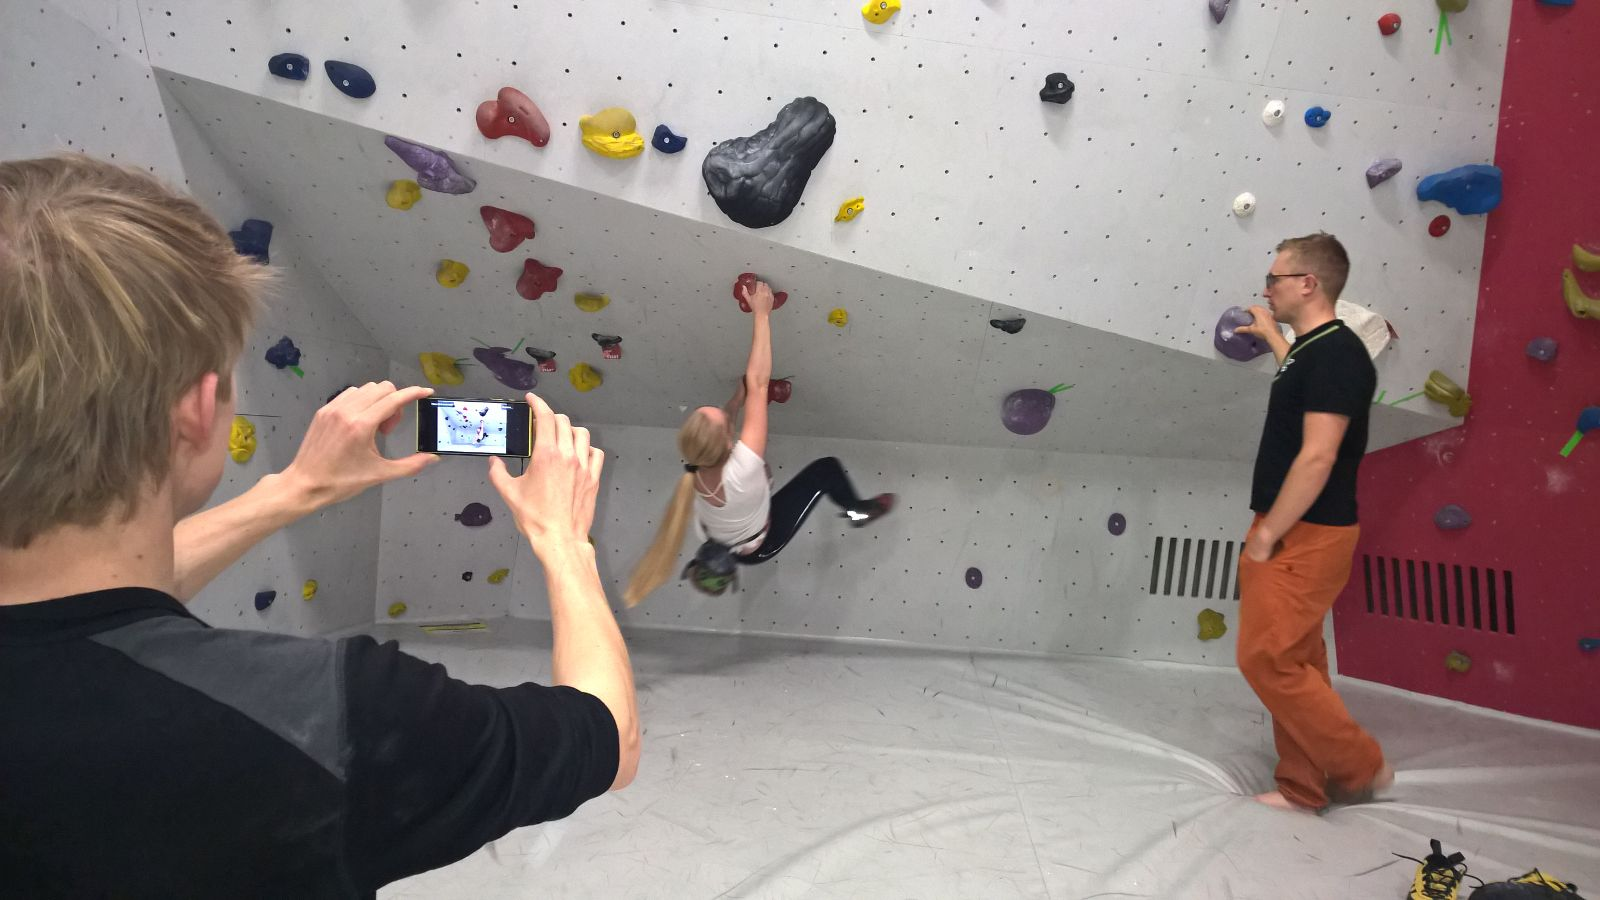
\includegraphics[width=\textwidth]{figures/images/Live-Video.jpg}
        \caption{A camera operator with a smartphone, and climber, wearing a Google Glass.}
        \label{fig:live-video-action}
    \end{subfigure}
    \caption{The live video setup, utilizing a smartphone and a pair of smart glasses.}
    \label{fig:live-video}
\end{figure}
